\documentclass{beamer}

\setbeamertemplate{navigation symbols}{}

\usepackage{xcolor}
\usepackage{tikz}
\usepackage{hyperref}
\usepackage{lmodern}

\title{Quantum phase estimation \\-\\ An example from chemistry}

\begin{document}
\frame{\titlepage}

\begin{frame}
\frametitle{prequisite: quantum circuits}

\begin{center}
\begin{figure}
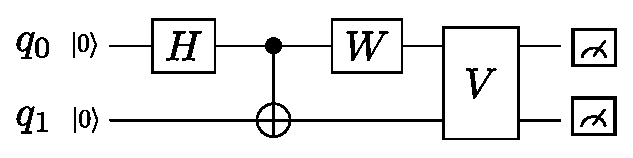
\includegraphics[width=0.6\textwidth]{quantum_circuit_example.eps}
\end{figure}
\end{center}
\begin{itemize}
\item qubit: 2-level quantum system ($|0\rangle, |1\rangle$). \\ quantum computer = $n$ qubits.
\item quantum circuit $\simeq$ quantum program $=$ list of quantum instructions/gates.
\item The circuit above computes: $|\psi\rangle = V \cdot (W\otimes I) \cdot CNOT_{0\rightarrow 1} \cdot (H\otimes I) |00\rangle$
\end{itemize}

\begin{tikzpicture}
\node (text) at (0,0) {\textbf{Note:} ``controlled-gates'' means:};
\node (draw) at (6,0) {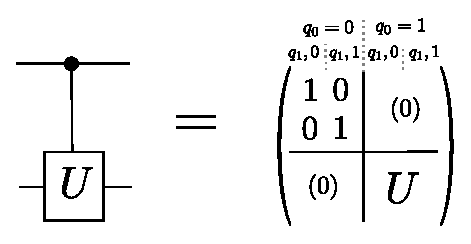
\includegraphics[width=.5\textwidth]{gate_example.eps}};
\end{tikzpicture}
 
\end{frame}

\begin{frame}
\frametitle{quantum phase estimation: original form}
\begin{center}
\begin{figure}
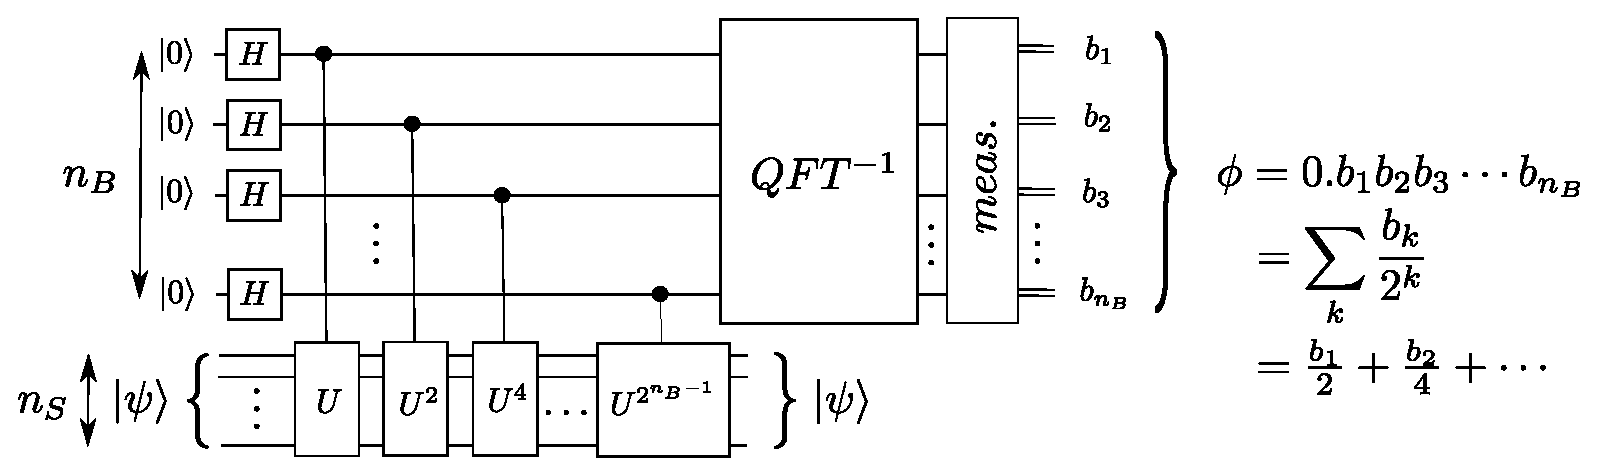
\includegraphics[width=\textwidth]{quantum_phase_estimation.eps}
\end{figure}
\end{center}

With $|\psi\rangle$ \textbf{eigenvector} of $U$ with \textbf{eigenvalue} $e^{-2i\pi\phi}$,\\~\\
 ($U|\psi\rangle = e^{-2i\pi\phi}|\psi\rangle$, $0\leq\phi<1$)\\~\\
The circuit above allows to compute the $n_{B}$ most significant bits of $\phi$ in a \textbf{binary
decomposition}.\\~\\

\textbf{Template} for \emph{all} quantum algorithms with \textbf{exponential speedup}.\\
(i.e with quantum circuits of \textbf{polynomial} size for classically-intractable problems)
\end{frame}

\begin{frame}
\frametitle{iterative quantum phase estimation: what we will use}

{\fontfamily{lmr}\selectfont for k in \textbf{range}($n_{B}$, 0, -1)\footnote{Python style}:
\begin{itemize}
\item[1.] compute $\phi_{k}=\sum_{l=k+1}^{n_{B}} \frac{b_{l}}{2^{l-k+1}}$
\item[2.] execute the following circuit: 
\end{itemize}
}
\begin{figure}
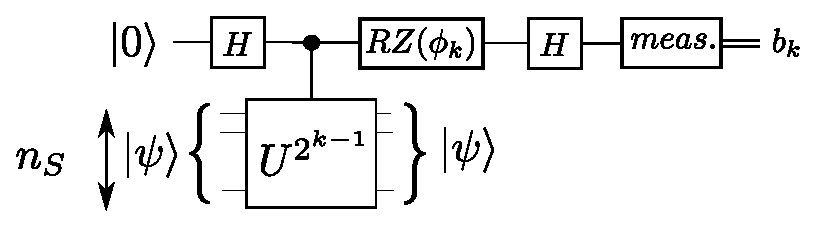
\includegraphics[width=.6\textwidth]{iterative_pea.eps}
\end{figure}~\\

With $H=\frac{1}{\sqrt{2}}\begin{pmatrix}1 & 1 \\ 1 & -1 \end{pmatrix}$ and 
$RZ(\phi_{k})=\begin{pmatrix} 1 & 0 \\ 0 & e^{i\phi_{k}}\end{pmatrix}$

\end{frame}

\begin{frame}
\begin{center}
\begin{figure}
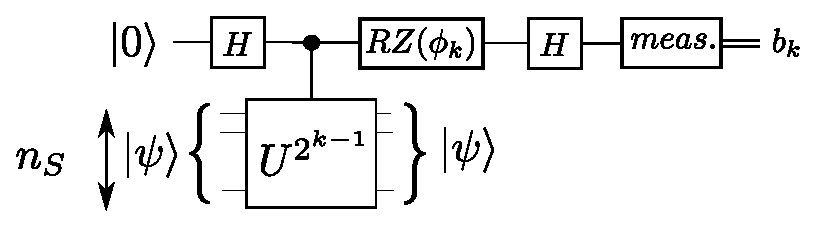
\includegraphics[width=.6\textwidth]{iterative_pea.eps}
\end{figure}
\end{center}
Recall that $\phi=0.b_{1}\cdots b_{n_{B}}$ in binary decomposition 
and $\phi_{k}=\sum_{l=k+1}^{n_{B}} \frac{b_{l}}{2^{l-k+1}}=0.0b_{k+1}\cdots b_{n_{B}}$.\\~\\
\textbf{Evolution of the system:}\\~\\
$|0\rangle|\psi\rangle \underset{H}{\rightarrow} \left(\frac{|0\rangle+|1\rangle}{\sqrt{2}}\right)|\psi\rangle=
\left(\frac{|0\rangle|\psi\rangle+|1\rangle|\psi\rangle}{\sqrt{2}}\right)$\\~\\
$\underset{\bullet-U}{\hookrightarrow}\left(\frac{|0\rangle|\psi\rangle+e^{-2i\pi\cdot 2^{k-1}\phi}|1\rangle|\psi\rangle}{\sqrt{2}}\right)
=\left(\frac{|0\rangle+e^{-2i\pi\cdot 0.b_{k}\cdots b_{n_{B}}}|1\rangle}{\sqrt{2}}\right)|\psi\rangle$\\~\\
$\underset{RZ(\phi_{k})}{\hookrightarrow} \left(\frac{|0\rangle+e^{-2i\pi\cdot 0.b_{k}}|1\rangle}{\sqrt{2}}\right)|\psi\rangle
=\left(\frac{|0\rangle+(-1)^{b_{k}}|1\rangle}{\sqrt{2}}\right)|\psi\rangle
\underset{H}{\rightarrow}|b_{k}\rangle|\psi\rangle$
\end{frame}

\begin{frame}
\frametitle{Our use-case: ground state energy calculation}
Given $\mathcal{H}$, Hamiltonian of target system (e.g a molecule), we want to compute its ground state energy.\\~\\
Actually, usually $\mathcal{H}$ depends on some structural/geometric parameters (e.g $H_{2}$ dissociation curve). The purpose
is then to compute a \emph{ground state energy landscape} as a function of these parameters. May provide insight on reaction mechanisms
\footnote{Potential futuristic applications: $CO_{2}$ capture 
\textcolor{blue}{\cite{von2020quantum}}, $H_{2}O$ cracking...}.
\begin{center}
\begin{tikzpicture}
\node (molecule) at (0,0) {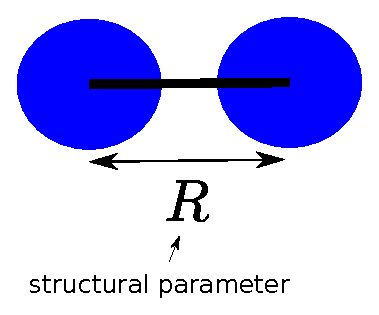
\includegraphics[width=.2\textwidth]{di_hydrogen.eps}};
\node (arrow) at (2,0) {$\rightarrow$};
\node (curve) at (5,0) {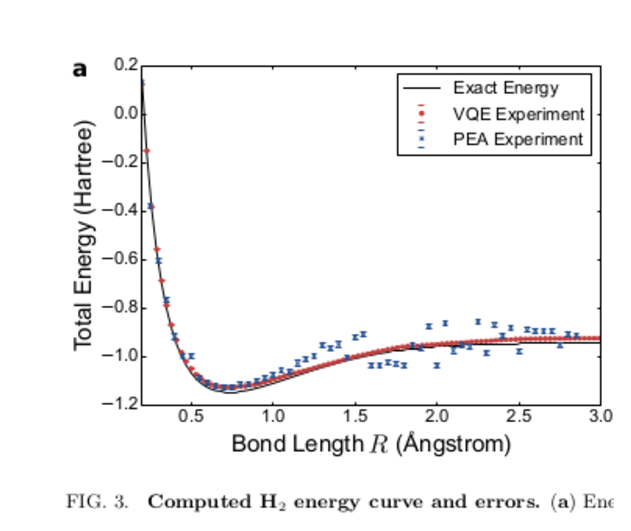
\includegraphics[width=.3\textwidth]{dissociation_curve.eps}};
\end{tikzpicture}
\end{center}

From \textcolor{blue}{\cite{o2016scalable}}. This is what we will reproduce today.
\end{frame}

\begin{frame}

\begin{center}
\begin{figure}
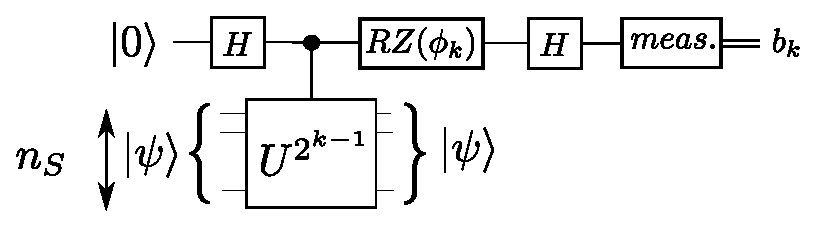
\includegraphics[width=.6\textwidth]{iterative_pea.eps}
\end{figure}
\end{center}

We will therefore work with:
\begin{itemize} 
\item $U=e^{-i\mathcal{H}dt}$, for some value of $dt$ to be chosen.
\item $|\psi\rangle$ the ground state of $H$, whose energy $E$ we want to compute.
\item we then have $U|\psi\rangle = e^{-iEdt}|\psi\rangle= e^{-2i\pi\frac{Edt}{2\pi}}$
\end{itemize}
------\\
\textbf{Problem 1:} the algorithm only allows us to compute $\phi=\frac{Edt}{2\pi}\: \text{mod}\: \left[1\right]$ ($\in \left[0,1\right]$)\\~\\
Following \textcolor{blue}{\cite{whitfield2011simulation}}, we will use an \emph{interval guess} $\left[E_{min},E_{max}\right]$ 
for $E$.\\
Then $\mathcal{H}\leftarrow \mathcal{H}-E_{min}\cdot I$ ensures $E>0$ and choosing $dt=\frac{2\pi}{E_{max}}$ ensures $\frac{Edt}{2\pi}<1$ 

\end{frame}

\begin{frame}
\frametitle{Other problems}
\textbf{Problem 2} In general we do not have access to the ground state.\\$\quad\rightarrow$use an \textbf{ansatz}\footnote{easy-to-prepare approximation} 
with theoretical good overlap with ground state.\\~\\

\textbf{Problem 3} How do we implement $U^{2^{k}} = e^{-i\mathcal{H}2^{k}dt}$ ?\\
$\quad\rightarrow$ usually $\mathcal{H}$ comes as a sum of simpler terms $\sum_{l} \mathcal{H}_{l}$\\
$\quad$(e.g Pauli products) for which $e^{-i\mathcal{H}_{l}dt}$ is simple to implement.\\
$\quad\rightarrow$ and use \textbf{Trotter's formula} \textcolor{blue}{\cite{whitfield2011simulation}} 
$$ e^{-i\left(\sum_{l}\mathcal{H}_{l}\right)dt} \simeq \left(\prod_{l} e^{-\frac{i\mathcal{H}_{l}dt}{p} }\right)^{p} $$ 

with $p$ integer, as large as possible.

\end{frame}

\begin{frame}
\begin{itemize}
\item We will reproduce the curves from \textcolor{blue}{\cite{o2016scalable}}.
\item In this example: 
    \begin{itemize}
    \item $n_{S}=2$
    \item $H(R) = g_{0}I+g_{1}ZI+g_{2}IZ+g_{3}ZZ+g_{4}YY+g_{5}XX$\footnote{This Hamiltonian is the output of (1) a conversion from an \emph{electronic structure Hamiltonian} to a \emph{spin Hamiltonian} expressed with Pauli matrices and (2) simplifications leveraging theoretical chemistry knowledge}
    \item The coefficients are stored in {\fontfamily{lmr}\selectfont hamiltonian\_data.json}
    \end{itemize}
\item The purpose is to reproduce
\begin{center}
\begin{figure}
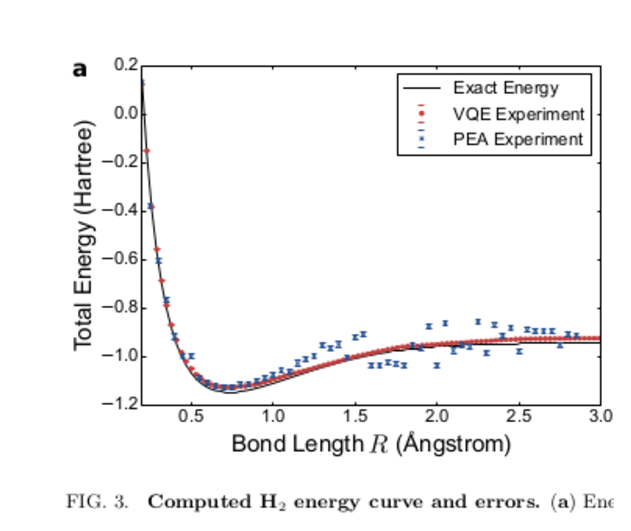
\includegraphics[width=.5\textwidth]{dissociation_curve.eps}
\end{figure}
\end{center}
\end{itemize}
\end{frame}

\begin{frame}
\frametitle{The programming framework we will use: myqlm}

What you need to know:
\begin{itemize}
\item quantum circuits are first written as \textbf{Program} and then exported as \textbf{circuit}.
\item A \textbf{job} is created from a circuit and sent to a \textbf{qpu} (a simulator)
\item \textbf{AbstractGates} will come handy in programming Hamiltonian simulation.
\item see the minimal notebook and \textcolor{blue}{\href{https://myqlm.github.io/}{https://myqlm.github.io/}} for more details
\end{itemize}

\end{frame}

\bibliographystyle{unsrt}
\bibliography{biblio}
\end{document}
